\documentclass[11pt,letterpaper]{article}

% ======================================================================
% 1. Page Geometry
% ======================================================================
\usepackage[margin=1in]{geometry}

% ======================================================================
% 2. Mathematics, Theorems & Fonts (load ams before newtx; keep amssymb/amsthm)
% ======================================================================
\usepackage[T1]{fontenc}
\usepackage[utf8]{inputenc}
\usepackage{amsmath,amssymb,amsthm}
\let\Bbbk\relax
\let\openbox\relax
\usepackage{newtxtext,newtxmath}
\usepackage[expansion=false]{microtype}

\theoremstyle{plain}
\newtheorem{proposition}{Proposition}

% ======================================================================
% 4. Tables, Figures, TikZ & Lists
% ======================================================================
\usepackage{graphicx}
\usepackage{booktabs}
\usepackage{siunitx}
\usepackage{tabularx}
\usepackage{array}
\usepackage{caption}
\usepackage{subcaption}
\usepackage{enumitem}
\usepackage{tikz}
\usetikzlibrary{arrows.meta,positioning}

\sisetup{
  reset-text-series=false,
  text-series-to-math=true,
  reset-math-version=false,
  detect-all,
  mode=math,
  group-digits=integer,
  group-separator={,},
  group-minimum-digits=4,
}

\captionsetup{font=small,labelfont=bf}
\setlist[itemize]{leftmargin=1.4em,itemsep=1.2pt,topsep=2pt,parsep=0pt}
\setlist[enumerate]{leftmargin=1.5em,itemsep=1.2pt,topsep=2pt,parsep=0pt}
\setlength{\textfloatsep}{8.5pt plus 2pt minus 2pt}
\setlength{\floatsep}{7pt plus 2pt minus 2pt}
\setlength{\intextsep}{8.5pt plus 2pt minus 2pt}

% ======================================================================
% 4. Accent Palette (Used ONLY for Headings & Links), Headings, Bib & TODOs
% ======================================================================
\usepackage{xcolor}
\definecolor{DeepBlue}{HTML}{16324F}

\usepackage{titlesec}
\titleformat{\section}{\large\bfseries\color{DeepBlue}}{\thesection}{0.6em}{}
\titleformat{\subsection}{\normalsize\bfseries\color{DeepBlue}}{\thesubsection}{0.5em}{}
\titlespacing*{\section}{0pt}{1.15ex plus 0.2ex minus 0.1ex}{0.35ex plus 0.1ex}
\titlespacing*{\subsection}{0pt}{0.85ex plus 0.15ex minus 0.1ex}{0.25ex plus 0.1ex}

\usepackage[numbers,sort&compress]{natbib}
\setlength{\marginparwidth}{0.82in}
\usepackage[
  colorinlistoftodos,
  backgroundcolor=black!4,
  bordercolor=black!35,
  linecolor=black!35,
  textsize=tiny
]{todonotes}

% ======================================================================
% 5. Hyperlinks, Identifiers & Cross-Referencing (cleveref MUST load last)
% ======================================================================
\usepackage[
  colorlinks=true,
  linkcolor=DeepBlue,
  citecolor=DeepBlue,
  urlcolor=DeepBlue,
  pdftitle={Dialectical Counter-Anchoring Eliminates Social Herding That Nearly Doubles Homogeneous LLM Crowd Error},
  pdfauthor={Vikram Viswanath}
]{hyperref}

\makeatletter
\g@addto@macro\UrlBreaks{\do\_\do\-\do\.\do\/}
\makeatother
\newcommand{\code}[1]{\nolinkurl{#1}}
\newcommand{\taskid}[1]{\texttt{\small\hyphenpenalty=50 #1}}

\usepackage[capitalise,nameinlink,noabbrev]{cleveref}
\crefname{appendix}{Appendix}{Appendices}
\Crefname{appendix}{Appendix}{Appendices}

% Custom title & author block for clean Page 1 layout
\title{\Large\bfseries\color{DeepBlue}
  Dialectical Counter-Anchoring Eliminates Social Herding That Nearly Doubles Homogeneous LLM Crowd Error}

\author{
  Vikram Viswanath$^{1}$\thanks{Corresponding author (\texttt{svikramvish@gmail.com}). Research conducted at the \href{https://apartresearch.com/sprints/ai-x-epistemics-research-sprint-2026-11-13-to-2026-11-15}{AI $\times$ Epistemics Research Sprint}, Apart Research (November 2026); open track context per repository README (Track~4). Code and archives: \url{https://github.com/vikramwish/apart-epistemics} (branch \code{numeric-question-bank}, commit \texttt{3a6294c}).}\\[0.25em]
  \small $^{1}$Independent Researcher \quad $\cdot$ \quad Research conducted at the AI $\times$ Epistemics Research Sprint, Apart Research
}
\date{}

\begin{document}
\maketitle
\thispagestyle{plain}

\begin{abstract}
\noindent
Multi-agent forecasting and reasoning systems increasingly pair large language model (LLM) assistants with peer consensus summaries such as group medians and interquartile ranges. When agents share a foundation model or absorb unexamined peer anchors, correlated biases and repeated feedback can amplify error and undermine collective safety. In this work, we show that consensus telemetry degrades homogeneous LLM accuracy whereas explicit dialectical counter-anchoring eliminates this failure across 1,280 controlled agent-round responses spanning 16 scientific estimation tasks, eight agents ($\alpha = 0.4$), and five conditions. Specifically, holding the backbone model fixed (\texttt{gemma-4-26b-a4b-it}), revealing peer medians nearly doubles Round-2 squared $\log_{10}$ crowd error relative to isolated estimation ($0.011944 \to 0.022899$, $+91.7\%$, exact Wilcoxon $p = 0.005371$, Holm-adjusted $p = 0.032227$), while prepending a 53-word prompt refuting both overshoot and undershoot errors cuts error by $48.4\%$ to $0.011818$ ($p = 0.001099$) across all 16 leave-one-task-out drops. Leveraging an exact variance decomposition and cross-round identity, we further show that combining four architectures with counter-anchoring achieves lower crowd error ($0.007692$) sub-additively (interaction $= +0.008715$, Holm $p = 0.000916$) by reducing positive cross-round error covariance by $68\%$. Finally, we analyze task-level permutation nulls and constituent model error, finding that combined four-model intervention over naive mixing is non-significant after multiplicity control ($p = 0.127869$) and remains confounded with stronger constituent models until implemented controls run. These results establish naive social telemetry as an epistemic hazard in shared-model collectives and concise counter-anchoring as an auditable guardrail.
\end{abstract}

\noindent\textbf{Keywords:} algorithmic monoculture, social herding, dialectical counter-anchoring, cognitive forcing, multi-agent epistemics\todo{Confirm portal track matches \code{README.md} Track~4.}

% ======================================================================
\section{Introduction}
% ======================================================================

Forecasting teams, collaborative assistants, and multi-agent pipelines increasingly combine large language model (LLM) outputs with live social consensus statistics such as group medians, interquartile ranges (IQRs), and shared dashboards. When participants query instances of the same model family---or when assistants condition directly on group telemetry---two linked risks threaten AI-assisted epistemics. First, \emph{algorithmic monoculture} correlates failure modes across ostensibly independent agents~\citep{kleinberg2021algorithmic,kim2025correlated,jiang2025artificial}. Second, \emph{AI-mediated social herding} arises when assistants reinforce peer anchors rather than offering an independent physical check, compounding errors across iterative updates~\citep{demarzo2003persuasion,denisov2026consensus}. Separating reliable protocol fixes from confounding model swaps is therefore essential before deploying multi-agent estimation interfaces in safety-critical settings.

In this work, we evaluate how consensus telemetry, dialectical cognitive forcing, and multi-architecture panels shape Round-2 $\log_{10}$ mean squared error (MSE) over 1,280 agent-round evaluations ($1,318$ logged provider calls) across five conditions (\texttt{P0}--\texttt{P4}), previewed in~\cref{fig:headline}. Following a post-run audit of raw API traces and permutation nulls, our paper makes four verified contributions mirroring our abstract:
\begin{itemize}
  \item \textbf{Unconfounded causal identification (\texttt{P0}--\texttt{P2}):} Holding \texttt{gemma-4-26b-a4b-it} strictly fixed across $N=8$ agents, showing peer median and IQR telemetry (\texttt{P1}) worsens Round-2 crowd MSE by $+91.7\%$ over isolated estimation (\texttt{P0}), while our 53-word dialectical counter-anchoring protocol (\texttt{P2}) cuts crowd MSE by $-48.4\%$ and survives all 16 leave-one-task-out (LOTO) exclusions.
  \item \textbf{Hierarchical variance and null accounting:} Combining~\citet{krogh1995neural} and~\citet{page2007difference} with one-way ANOVA partitions crowd diversity into $D_{\text{within}} + D_{\text{between}}$, paired with an exact finite-population permutation baseline ($\mathbb{E}_{\text{null}}[D_{\text{between}} \mid y] = 0.75\,\mathbb{E}_{\text{null}}[D_{\text{within}} \mid y]$ for $N=8, K=4$).
  \item \textbf{Sub-additive interaction and covariance mechanism:} Crossing four model families (\texttt{P3}, \texttt{P4}) with counter-anchoring reveals strong sub-additivity (difference-in-differences $\text{DiD}=+0.008715$, Holm $p_{\text{H5}}=0.000916$) and explains via an exact cross-round identity why \texttt{P4} outperforms \texttt{P3} on blended error despite higher raw Round-2 assistant MSE.
  \item \textbf{Open-box provenance and causal boundary:} We disclose all 28 Wave-1 trajectory replacements, 14 length truncations at the runtime $8,192$-token floor, single-task leverage on \taskid{hyd\_lake\_superior\_vol\_km3}, non-significance of \texttt{P4} vs.\ \texttt{P3} ($p_{\text{H9}}=0.127869$), and capability confounding addressed by three implemented controls.
\end{itemize}

\begin{figure}[t]
  \centering
  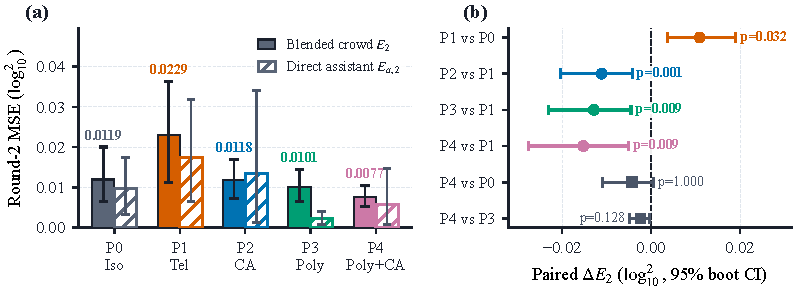
\includegraphics[width=0.92\textwidth]{figures/fig1_headline_herding.pdf}
  \caption{\textbf{Peer telemetry degrades fixed-model crowd accuracy, while dialectical counter-anchoring and multi-architecture panels mitigate herding.} \textbf{(a)}~Round-2 blended crowd MSE ($E_2$, solid bars) and direct assistant MSE ($E_{a,2}$, hatched) across \texttt{P0}--\texttt{P4}; error bars denote 2,000-resample task-level bootstrap $95\%$ confidence intervals ($n=16$ tasks). \textbf{(b)}~Pre-specified paired task contrasts ($\Delta E_2$) with bootstrap $95\%$ CIs and exact $m=9$ Holm-adjusted $p$-values ($n_{\text{nz}}=15$).}
  \label{fig:headline}
\end{figure}

% ======================================================================
\section{Related Work}
% ======================================================================

\paragraph{Algorithmic Monoculture and Homogenization.}
\citet{kleinberg2021algorithmic} formalized how algorithmic monoculture induces correlated mistakes that reduce collective welfare even when individual models are accurate. Empirically, LLM assistance narrows lexical and content diversity~\citep{padmakumar2024writing,sourati2026shrinking}, homogenizes open-ended outputs~\citep{jiang2025artificial,qiu2026revisiting,schaeffer2026reevaluating}, and flattens public debate~\citep{kim2026argument,thejaswi2026linguistic}. Crucially,~\citet{kim2025correlated} documented cross-lab error correlations across 350+ models, while~\citet{peterson2024knowledge} and~\citet{fu2026beyond} highlighted long-run knowledge collapse and decoding convergence. Unlike single-turn stylistic studies, we audit ground-truth MSE across iterative belief pooling.

\paragraph{Social Influence and Multi-LLM Ensembles.}
Boundedly rational networks amplify double-counted rumors through persuasion bias~\citep{demarzo2003persuasion,goldman2001experts}, a failure observed when LLM societies form shared conventions or polarize~\citep{centola2018experimental,ashery2025emergent,chuang2023simulating,wynn2025talk,estornell2024multillm}. Conversely, \emph{static} cross-model aggregation can rival human forecasting tournaments~\citep{schoenegger2024silicon} and crowd-decoding aids numeric guesstimation~\citep{chuang2025probing}, whereas naive multi-agent debate often underperforms self-consistency unless disagreement is structured~\citep{smit2024mad,schneider2025wisdom,wang2024moa,denisov2026consensus,quattrociocchi2025epistemological}.

\paragraph{Cognitive Forcing and Deference.}
In human--AI teaming,~\citet{bucinca2021trust} showed that cognitive forcing functions curtail passive deference to anchors. Within LLMs, unguided self-correction fails without external or adversarial structure~\citep{huang2024selfcorrect,liang2024encouraging,taubenfeld2024systematic}, and sycophancy undermines epistemic independence~\citep{sharma2024sycophancy,kelley2026personalization,deepthika2026sycophancy,finnveden2024epistemics}. Our dialectical counter-anchoring instruction applies a two-sided forcing prompt explicitly targeting both the agent's own prior and the group median.

% ======================================================================
\section{Methods}
% ======================================================================

\subsection{Hierarchical Page ANOVA and Cross-Round Error Identities}

For each quantitative benchmark task $q$ with positive reference truth $T_q > 0$, errors are scored in $\log_{10}$ space around $y_q^\star = \log_{10}(T_q)$. A population of $N=8$ agents partitioned into $K$ model families $\mathcal{G}_1,\dots,\mathcal{G}_K$ ($n_k = |\mathcal{G}_k|$, $\sum_k n_k = N$) starts at seeded Round-0 estimates $x_{i,0}$. At rounds $t \in \{1,2\}$, agent $i$ queries an assistant producing parsed $\log_{10}$ output $a_{i,t}$ and updates via boundedly rational linear pooling ($\alpha = 0.4$):
\begin{equation}\label{eq:update-rule}
  x_{i,t} = (1-\alpha)\,x_{i,t-1} + \alpha\,a_{i,t} = 0.6\,x_{i,t-1} + 0.4\,a_{i,t}.
\end{equation}
Unrolling~\eqref{eq:update-rule} gives $x_{i,2} = 0.36\,x_{i,0} + 0.24\,a_{i,1} + 0.40\,a_{i,2}$, where $0.36$ is the initial prior's direct weight ($0.36^2 = 12.96\%$ squared coefficient, distinct from its empirical covariance-inclusive variance share). Denote crowd mean $\bar{x}_t = N^{-1}\sum_i x_{i,t}$, family means $\bar{x}_{k,t} = n_k^{-1}\sum_{i\in \mathcal{G}_k} x_{i,t}$, crowd error $E_t = (\bar{x}_t - y^\star)^2$, individual MSE $\bar{e}_t = N^{-1}\sum_i (x_{i,t}-y^\star)^2$, and direct assistant equivalents $E_{a,t}, \bar{e}_{a,t}$. We also report the Error-to-Variance Retention Ratio $\text{EVRR}_t = D_t / \bigl((1-\alpha)^2 D_{t-1}\bigr)$ comparing realized diversity against passive shrinkage.

\begin{proposition}[Hierarchical Page ANOVA Identity]\label{prop:hier-page}
Extending the ensemble ambiguity decomposition~\citep{krogh1995neural,page2007difference} with one-way ANOVA across $K$ groups of equal size $n=N/K$, let $D = N^{-1}\sum_{i=1}^N (y_i - \bar{y})^2$ ($y_i=x_{i,t}$ or $a_{i,t}$). Then
\begin{equation}\label{eq:hier-page}
  E = \bar{e} - \bigl(D_{\text{within}} + D_{\text{between}}\bigr), \quad
  D_{\text{within}} = \frac{1}{N}\sum_{k=1}^K \sum_{i\in \mathcal{G}_k}(y_i - \bar{y}_k)^2, \quad
  D_{\text{between}} = \frac{1}{N}\sum_{k=1}^K n_k(\bar{y}_k - \bar{y})^2.
\end{equation}
Under uniform random permutation of fixed values $\{y_1,\dots,y_N\}$ across the $K$ group labels, conditional expectations obey
\begin{equation}\label{eq:perm-null}
  \mathbb{E}_{\text{null}}\bigl[D_{\text{between}} \mid y\bigr] = \frac{K-1}{N-K}\,\mathbb{E}_{\text{null}}\bigl[D_{\text{within}} \mid y\bigr],
\end{equation}
yielding $\mathbb{E}_{\text{null}}[D_{\text{between}} \mid y] = 0.75\,\mathbb{E}_{\text{null}}[D_{\text{within}} \mid y]$ and zero-expectation excess divergence $D_{\text{excess}} = D_{\text{between}} - 0.75\,D_{\text{within}}$ for $(N,K)=(8,4)$.
\end{proposition}
\begin{proof}[Proof sketch]
Centered ANOVA yields $D = D_{\text{within}} + D_{\text{between}}$ because cross-terms $\sum_{i\in\mathcal{G}_k}(y_i - \bar{y}_k)(\bar{y}_k - \bar{y})$ vanish. Simple random sampling without replacement of size $n$ from variance $S^2 = \frac{N}{N-1}D$ gives $\mathbb{E}_{\text{null}}[D_{\text{within}} \mid y] = \frac{K(n-1)}{N}S^2 = \frac{N-K}{N-1}D$, leaving $\mathbb{E}_{\text{null}}[D_{\text{between}} \mid y] = \frac{K-1}{N-1}D$. Their ratio establishes~\eqref{eq:perm-null}.
\end{proof}

Crucially, positive $D_{\text{excess}}$ alone does not prove systematic model specialization; we therefore enumerate all $8!/((2!)^4 4!) = 105$ unlabeled partitions per task. Furthermore, averaging~\eqref{eq:update-rule} yields an exact signed-error decomposition separating Round-1 carry, Round-2 assistant error, and cross-round covariance:
\begin{equation}\label{eq:cross-term}
  E_2 = 0.36\,E_1 + 0.16\,E_{a,2} + 0.48\,(\bar{x}_1 - y^\star)(\bar{a}_2 - y^\star).
\end{equation}

\subsection{Experimental Protocol and Simulation Pipeline}

As illustrated in~\cref{fig:pipeline} and detailed in~\cref{tab:conditions}, all five arms initialize identical Round-0 priors from $x_{i,0} \sim \mathcal{N}(y_q^\star + 0.22\,b_q,\, 0.24^2)$ (\texttt{seed=42}, misconception polarity $b_q \in \{-0.8, +0.8\}$, Round-0 crowd MSE $E_0 = 0.048728$). Only \texttt{P0}, \texttt{P1}, and \texttt{P2} hold the assistant fixed (\texttt{gemma-4-26b-a4b-it}), yielding clean single-factor identification for peer telemetry (\texttt{P1} vs.\ \texttt{P0}) and counter-anchoring (\texttt{P2} vs.\ \texttt{P1}). Polyphonic arms \texttt{P3} and \texttt{P4} allocate two seats each to \texttt{gemma-4-26b-a4b-it}, \texttt{deepseek-v4-flash}, \texttt{qwen3.8-27b}, and \texttt{glm-5.2}. Logged HTTP requests omit \texttt{temperature} and \texttt{top\_p} (using API provider defaults) with \texttt{reasoning=\{"effort":"none"\}} on the three reasoning-capable endpoints. User prompts format numbers via \code{format\_prompt\_number} (3 significant figures) and enforce \code{MAX\_LOG10\_JUMP = 2.0} before single-retry reprompting; verbatim prompts appear in~\cref{app:prompts}.

\begin{figure}[t]
  \centering
  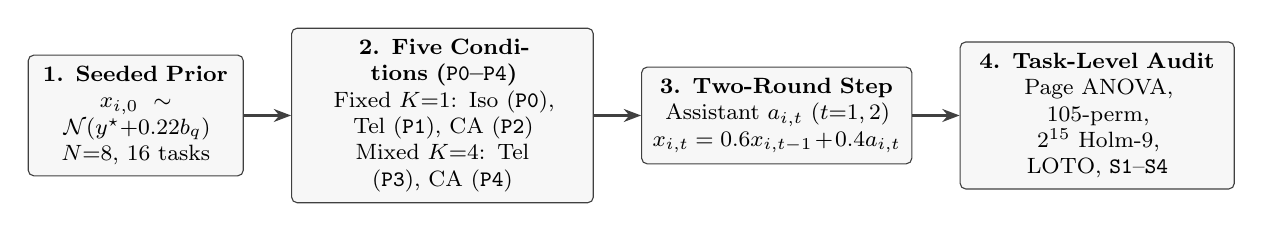
\begin{tikzpicture}[
    font=\footnotesize,
    node distance=5mm and 6mm,
    box/.style={draw=black!75, rounded corners=2pt, fill=black!3, align=center, inner sep=4pt, minimum height=9.5mm},
    arrow/.style={-{Stealth[length=2.2mm]}, thick, draw=black!75}
  ]
    \node[box, text width=2.45cm] (seed) {\textbf{1. Seeded Prior}\\$x_{i,0} \sim \mathcal{N}(y^\star{+}0.22b_q)$\\$N{=}8$, $16$ tasks};
    \node[box, right=of seed, text width=3.55cm] (conds) {\textbf{2. Five Conditions (\texttt{P0}--\texttt{P4})}\\Fixed $K{=}1$: Iso (\texttt{P0}), Tel (\texttt{P1}), CA (\texttt{P2})\\Mixed $K{=}4$: Tel (\texttt{P3}), CA (\texttt{P4})};
    \node[box, right=of conds, text width=3.15cm] (loop) {\textbf{3. Two-Round Step}\\Assistant $a_{i,t}$ ($t{=}1,2$)\\$x_{i,t} = 0.6 x_{i,t-1} + 0.4 a_{i,t}$};
    \node[box, right=of loop, text width=3.20cm] (audit) {\textbf{4. Task-Level Audit}\\Page ANOVA, 105-perm,\\$2^{15}$ Holm-9, LOTO, \texttt{S1}--\texttt{S4}};
    \draw[arrow] (seed) -- (conds);
    \draw[arrow] (conds) -- (loop);
    \draw[arrow] (loop) -- (audit);
  \end{tikzpicture}
  \caption{\textbf{End-to-end simulation and audit pipeline across \texttt{P0}--\texttt{P4}.} Identically seeded priors update through two sequential rounds ($\alpha=0.4$) and feed deterministic hierarchical variance, sign-flip permutation, and leave-one-task-out audits.}
  \label{fig:pipeline}
\end{figure}

\begin{table}[t]
\centering
\caption{\textbf{Experimental design, model allocation, and API spend across \texttt{P0}--\texttt{P4}.} Only \texttt{P0}--\texttt{P2} hold the model constant; \texttt{P3}--\texttt{P4} cross architectural mixing with stronger constituent endpoints.}
\label{tab:conditions}
\footnotesize
\setlength{\tabcolsep}{4.5pt}
\begin{tabular}{@{}l c l l l S[table-format=3.1] S[table-format=3.1] S[table-format=1.4]@{}}
\toprule
\textbf{Cond.} & \textbf{$K$} & \textbf{Model Allocation ($N=8$)} & \textbf{Telemetry} & \textbf{Prompting} & \textbf{In Tok} & \textbf{Out Tok} & \textbf{Ret.\ \$} \\
\midrule
\texttt{P0} & 1 & $8\times$ \texttt{gemma-4-26b-a4b-it} & None & Neutral estimator & 131.4 & 268.2 & 0.0266 \\
\texttt{P1} & 1 & $8\times$ \texttt{gemma-4-26b-a4b-it} & Median + IQR & Neutral estimator & 163.7 & 423.8 & 0.0330 \\
\texttt{P2} & 1 & $8\times$ \texttt{gemma-4-26b-a4b-it} & Median + IQR & 53-wd Counter-Anchor & 233.8 & 333.4 & 0.0304 \\
\texttt{P3} & 4 & $2\times$\{\texttt{gemma-4}, \texttt{ds-v4}, \texttt{qwen3.8}, \texttt{glm-5.2}\} & Median + IQR & Neutral estimator & 148.7 & 487.3 & 0.1637 \\
\texttt{P4} & 4 & $2\times$\{\texttt{gemma-4}, \texttt{ds-v4}, \texttt{qwen3.8}, \texttt{glm-5.2}\} & Median + IQR & 53-wd Counter-Anchor & 219.5 & 562.1 & 0.2326 \\
\bottomrule
\end{tabular}
\end{table}

\subsection{Cold-Probed Benchmark and Statistical Analysis Plan}

To prevent cherry-picking, 24 candidate benchmarks were cold-probed across all four models before executing \texttt{P0}--\texttt{P4}, yielding 16 sampled tasks (\texttt{seed=42}) stratified across \code{high\_spread} ($n=6$), \code{low\_spread} ($n=6$), and \code{control} ($n=4$); exact institutional definitions appear in~\cref{app:benchmark}. Task-level inference ($n=16$ independent units) uses two-sided paired Wilcoxon signed-rank tests with Holm--Bonferroni control across pre-specified families defined in \code{numeric\_core.py} prior to execution at commit \texttt{b5b91ce}: $m=9$ primary pairwise comparisons, $m=5$ factorial DiD metrics, and an exploratory $m=20$ family, alongside 2,000-resample bootstrap $95\%$ CIs (\texttt{seed=42}). Because all 80 calls on \taskid{sci\_lhc\_dipole\_magnets\_count} output $1{,}232$ ($n_{\text{nz}}=15$ non-zero pairs), we report both exact $2^{15}$ sign-flip enumeration ($p_{\text{exact}}$) and continuity-corrected normal approximations ($p_{\text{pipe}}$). Three follow-up controls isolating silent four-model aggregation (\code{P0\_POLY}), neutral reflection length (\code{P1\_REFLECT}), and homogeneous frontier panels remain implemented yet unrun in \code{configs/polyphony\_controls.yaml}.

% ======================================================================
\section{Results}
% ======================================================================

\subsection{Execution Integrity and Open-Box Request Audit}

\noindent\textbf{All 1,280 retained evaluations match logged API payloads with exact algebraic closure ($1.39 \times 10^{-16}$ residual), and key findings survive restoring replaced Wave-1 calls.} Beyond the 1,280 retained rows (zero missing cells, zero hidden reasoning tokens, $\$0.486271$ retained spend), raw HTTP traces record 38 non-retained calls across 1,318 requests ($\$0.501372$ total spend): 28 Wave-1 cells overwritten at \texttt{23:28} during re-sampling on three tasks (\taskid{mat\_molybdenum\_\allowbreak melting\_c}, \taskid{nrg\_france\_\allowbreak nuclear\_2022\_twh}, \taskid{env\_ipcc\_\allowbreak 1750\_ch4\_ppb}), eight in-run retries, and two re-sample retries. Exactly 14 calls terminated with \code{finish\_reason="max\_output\_tokens"} at the runtime $8{,}192$-token floor in \code{providers.py} (overriding manifest \code{max\_tokens=1024}): 13 \texttt{gemma-4-26b-a4b-it} repetition loops and one \texttt{qwen3.8-27b} response. Restoring the 28 pre-23:28 cells (\taskid{First\_Pass\_\allowbreak Saved\_Pre2328}: Round-2 $E_2 = 0.011978$, $0.025049$, $0.012681$, $0.010058$, $0.007692$) preserves all confirmatory conclusions (\texttt{P1 vs P0} $p_{\text{H9,ex}}=0.02564$; \texttt{P2 vs P1} $0.02350$; \texttt{P3 vs P1} $0.00769$; \texttt{P4 vs P1} $0.00769$; DiD $+0.010002$, $p_{\text{ex}}=0.00537$), whereas the strictest unretried chronological baseline weakens only \texttt{P1 vs P0} ($p_{\text{H9,ex}}=0.18091$, \cref{app:audit}).

\subsection{Main Outcomes and Pre-Specified Contrasts}

\noindent\textbf{Homogeneous social telemetry nearly doubles Round-2 crowd error (\texttt{P1} vs.\ \texttt{P0}: $+91.7\%$), whereas counter-anchoring (\texttt{P2}: $-48.4\%$) and four-architecture panels (\texttt{P3}/\texttt{P4}) reverse the collapse while leaving \texttt{P4} vs.\ \texttt{P3} non-significant.} As shown in~\cref{fig:headline,tab:main-metrics,tab:contrasts,fig:hier-page}:
\begin{enumerate}
  \item \textbf{Social herding degrades fixed-model accuracy (\texttt{P1 vs P0}):} Surfacing peer medians inside homogeneous \texttt{gemma-4-26b-a4b-it} raises Round-2 crowd error from $0.011944$ to $0.022899$ ($+0.010955$, $13/16$ worse, exact $p=0.005371$, $p_{\text{H9,ex}}=0.032227$, $p_{\text{H9,pipe}}=0.049594$; exploratory $p_{\text{H20,ex}}=0.085938$). Total diversity falls $43.1\%$ ($0.016806 \to 0.009557$) and H4 prior slope $s_{\text{user}}$ drops from $0.1339$ to $0.0085$.
  \item \textbf{Dialectical counter-anchoring eliminates the penalty (\texttt{P2 vs P1}):} Our 53-word bidirectional critique block lowers crowd error by $-48.4\%$ ($0.022899 \to 0.011818$, $14/16$ improved, $p_{\text{H9,ex}}=0.001099$, $p_{\text{H20,ex}}=0.002441$), matching unsocial \texttt{P0} ($-0.000126$, $p_{\text{H9,ex}}=1.0$) with fewer mean output tokens than \texttt{P1} ($333.4$ vs.\ $423.8$).
  \item \textbf{Mixed panels beat \texttt{P1} but not \texttt{P0}, and \texttt{P4 vs P3} is non-significant:} Both \texttt{P3} ($0.010058$, $-56.1\%$) and \texttt{P4} ($0.007692$, $-66.4\%$) beat \texttt{P1} ($p_{\text{H9,ex}}=0.009277$; $p_{\text{H20,ex}}=0.022034$, $p_{\text{H20,pipe}}=0.054446$), yet neither beats \texttt{P0} ($p_{\text{H9,ex}}=1.0$) nor separates significantly from each other (\texttt{P4 vs P3}: $-23.5\%$, $13/16$ wins, $p_{\text{exact}}=0.025574$, $p_{\text{H9,ex}}=0.127869$). Stratum patterns hold across \code{high\_spread} (\texttt{P0}--\texttt{P4}: $0.01134$, $0.02157$, $0.01378$, $0.00967$, $0.00764$), \code{low\_spread} ($0.00641$, $0.01608$, $0.00828$, $0.00856$, $0.00621$), and \code{control} ($0.02115$, $0.03512$, $0.01419$, $0.01288$, $0.00999$).
\end{enumerate}

\begin{table}[t]
\centering
\caption{\textbf{Round-1 and Round-2 ($\log_{10}$ MSE) crowd error, Hierarchical Page decomposition, EVRR, and H4 user-prior slopes.} Task-mean vs.\ aggregate ratio definitions of between-model share appear in Footnote~$a$.}
\label{tab:main-metrics}
\scriptsize
\setlength{\tabcolsep}{2.4pt}
\begin{tabular}{@{}l c S[table-format=1.4] S[table-format=1.4] S[table-format=1.4] S[table-format=1.4] S[table-format=1.4] S[table-format=1.4] S[table-format=1.4] S[table-format=1.3] c@{}}
\toprule
\textbf{Arm} & \textbf{Rnd} & \textbf{$E$} & \textbf{$\bar{e}$} & \textbf{$D$} & \textbf{$D_{\text{win}}$} & \textbf{$D_{\text{btwn}}$} & \textbf{$D_{\text{ex}}$} & \textbf{$E_a$} & \textbf{EVRR} & \textbf{H4 $s_{\text{user}}$ [CI]} \\
\midrule
\texttt{P0} & R1 & 0.0195 & 0.0481 & 0.0286 & 0.0286 & 0.0000 & 0.0000 & 0.0191 & 1.282 & $0.126$ {\tiny[0.00,0.28]} \\
\texttt{P0} & R2 & \bfseries 0.0119 & 0.0288 & 0.0168 & 0.0168 & 0.0000 & 0.0000 & 0.0096 & 1.379 & $0.134$ {\tiny[0.00,0.29]} \\
\texttt{P1} & R1 & 0.0303 & 0.0556 & 0.0253 & 0.0253 & 0.0000 & 0.0000 & 0.0190 & 1.123 & --- \\
\texttt{P1} & R2 & 0.0229 & 0.0325 & 0.0096 & 0.0096 & 0.0000 & 0.0000 & 0.0173 & 1.070 & $0.009$ {\tiny[-.05,0.08]} \\
\texttt{P2} & R1 & 0.0193 & 0.0448 & 0.0255 & 0.0255 & 0.0000 & 0.0000 & 0.0229 & 1.159 & --- \\
\texttt{P2} & R2 & 0.0118 & 0.0247 & 0.0129 & 0.0129 & 0.0000 & 0.0000 & 0.0135 & 1.339 & $0.071$ {\tiny[0.00,0.15]} \\
\texttt{P3} & R1 & 0.0211 & 0.0440 & 0.0229 & 0.0114 & 0.0115 & 0.0029 & 0.0040 & 1.059 & --- \\
\texttt{P3} & R2 & 0.0101 & \bfseries 0.0191 & 0.0090 & 0.0042 & 0.0048 & 0.0017 & \bfseries 0.0023 & 1.106 & $-0.012$ {\tiny[-.09,0.06]} \\
\texttt{P4} & R1 & 0.0170 & 0.0429 & 0.0260 & 0.0108 & 0.0152 & 0.0071 & 0.0041 & 1.116 & --- \\
\texttt{P4} & R2 & \bfseries 0.0077 & 0.0215 & 0.0138 & 0.0048 & 0.0090 & 0.0054 & 0.0058 & 1.283 & $0.064$ {\tiny[-.01,0.17]} \\
\bottomrule
\end{tabular}
\par\vspace{2pt}
\raggedright\scriptsize
$^a$ Unweighted task-mean R2 $D_{\text{between}}/D$ share is $53.66\%$ (\texttt{P3}) and $47.41\%$ (\texttt{P4}) for agents ($57.72\%, 50.66\%$ assistants), versus aggregate-mean ratio $\bar{D}_{\text{between}}/\bar{D} = 53.68\%$ (\texttt{P3}) and $65.07\%$ (\texttt{P4}; assistants $70.81\%, 77.02\%$). Exact $E_2$ at 6 decimals: \texttt{P0} $0.011944$, \texttt{P1} $0.022899$, \texttt{P2} $0.011818$, \texttt{P3} $0.010058$, \texttt{P4} $0.007692$. Identity holds to $1.39\times 10^{-16}$.
\end{table}

\begin{table}[t]
\centering
\caption{\textbf{Pre-specified pairwise contrasts and $2\times 2$ Difference-in-Differences ($\mathrm{DiD} = (\texttt{P4}-\texttt{P3})-(\texttt{P2}-\texttt{P1})$) on Round-2 errors ($n=16$; $n_{\text{nz}}=15$).} Bold Holm entries satisfy $p < 0.05$.}
\label{tab:contrasts}
\scriptsize
\setlength{\tabcolsep}{2.8pt}
\begin{tabular}{@{}l S[table-format=-1.5] c c S[table-format=1.5] S[table-format=1.5] S[table-format=1.5] S[table-format=1.5]@{}}
\toprule
\textbf{Contrast} & \textbf{Mean Diff} & \textbf{Boot 95\% CI} & \textbf{W/L/T} & \textbf{$p_{\text{exact}}$} & \textbf{$p_{\text{pipe}}$} & \textbf{$p_{\text{H,ex}}$} & \textbf{$p_{\text{H,pipe}}$} \\
\midrule
\multicolumn{8}{@{}l}{\textit{Primary Agent Blended Crowd Error ($m=9$ Holm family)}} \\
\texttt{P1 vs P0} & +0.01096 & $[+0.00369, +0.01905]$ & 2/13/1  & 0.00537 & 0.00827 & \bfseries 0.03223 & \bfseries 0.04959 \\
\texttt{P2 vs P1} & -0.01108 & $[-0.02027, -0.00425]$ & 14/1/1  & 0.00012 & 0.00089 & \bfseries 0.00110 & \bfseries 0.00803 \\
\texttt{P3 vs P1} & -0.01284 & $[-0.02314, -0.00450]$ & 12/3/1  & 0.00116 & 0.00287 & \bfseries 0.00928 & \bfseries 0.02293 \\
\texttt{P4 vs P1} & -0.01521 & $[-0.02762, -0.00512]$ & 14/1/1  & 0.00116 & 0.00287 & \bfseries 0.00928 & \bfseries 0.02293 \\
\texttt{P4 vs P3} & -0.00237 & $[-0.00476, -0.00025]$ & 13/2/1  & 0.02557 & 0.02877 & 0.12787 & 0.14384 \\
\texttt{P4 vs P0} & -0.00425 & $[-0.01089, +0.00046]$ & 9/6/1   & 0.38940 & 0.37868 & 1.00000 & 1.00000 \\
\texttt{P4 vs P2} & -0.00413 & $[-0.00858, -0.00047]$ & 9/6/1   & 0.15143 & 0.14753 & 0.60571 & 0.59013 \\
\midrule
\multicolumn{8}{@{}l}{\textit{Raw Assistant Crowd Error ($m=9$ Holm family)}} \\
\texttt{P3 vs P1} & -0.01498 & $[-0.0297, -0.0040]$   & {---}   & 0.00153 & 0.00345 & \bfseries 0.01373 & \bfseries 0.03100 \\
\texttt{P4 vs P1} & -0.01154 & $[-0.0270, +0.0023]$   & {---}   & 0.07300 & 0.07360 & 0.51099 & 0.51521 \\
\texttt{P4 vs P3} & +0.00343 & $[-0.0026, +0.0111]$   & {---}   & 0.27686 & 0.27051 & 0.83106 & 0.81152 \\
\midrule
\multicolumn{8}{@{}l}{\textit{$2\times 2$ Interaction DiD ($m=5$ metric-family Holm)}} \\
\code{crowd\_error} & +0.00872 & $[+0.00349, +0.01581]$ & 1/14/1  & 0.00018 & 0.00109 & \bfseries 0.00092 & \bfseries 0.00546 \\
\code{asst\_crowd\_error} & +0.00726 & $[-0.00542, +0.02028]$ & 3/12/1 & 0.01245 & 0.01579 & \bfseries 0.04981 & 0.06314 \\
\bottomrule
\end{tabular}
\end{table}

\begin{figure}[t]
  \centering
  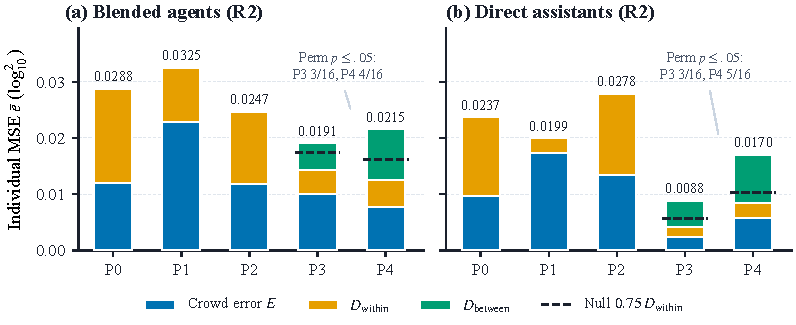
\includegraphics[width=0.92\textwidth]{figures/fig3_hierarchical_page.pdf}
  \caption{\textbf{Hierarchical Page decomposition confirms exact variance accounting while random-label permutation nulls temper diversity claims.} \textbf{(a)}~Blended agent and \textbf{(b)}~direct assistant MSE partitioned into crowd error $E$, $D_{\text{within}}$, and $D_{\text{between}}$ across \texttt{P0}--\texttt{P4} (identical $y$-axes). Dashed bars mark the random-label permutation null $0.75\,D_{\text{within}}$; exact 105-partition tests hit $p\le 0.05$ on only $3$--$5/16$ tasks.}
  \label{fig:hier-page}
\end{figure}

\subsection{Mechanistic Analysis, Capability Confounds, and Robustness}

\noindent\textbf{Cross-round covariance reduction drives \texttt{P4} below \texttt{P3} despite higher raw assistant error, while $16/16$ LOTO stability separates robust \texttt{P1} rescue from single-item leverage and capability confounds.}
Inspecting~\cref{fig:factorial,tab:mechanisms,fig:loto} establishes four mechanistic checks:
\begin{itemize}
  \item \textbf{Sub-additive interaction \& cross-round covariance:} Crossing mixing ($K \in \{1,4\}$) with counter-anchoring yields significant sub-additivity ($\text{DiD}=+0.008715$, $p_{\text{H5,ex}}=0.000916$, \cref{fig:factorial}a). Using~\eqref{eq:cross-term}, \texttt{P4} trails \texttt{P3} on $0.16 E_{a,2}$ ($0.000923$ vs.\ $0.000374$) yet outperforms \texttt{P3} on $E_2$ because \texttt{P4} lowers $0.36 E_1$ ($0.006105$ vs.\ $0.007599$) and cuts $0.48\,\text{Cross}$ by $68\%$ ($0.002085 \to 0.000664$, \cref{tab:mechanisms} left \& \cref{fig:loto}b), whereas \texttt{P1} accumulates $+0.009231$ positive covariance ($40.3\%$ of its total error).
  \item \textbf{Per-model capability confound:} Across $n=64$ retained responses per model inside \texttt{P3}--\texttt{P4} (\cref{fig:factorial}b, \cref{tab:mechanisms} right), \texttt{deepseek-v4-flash} ($0.00198 \to 0.00126$) and \texttt{glm-5.2} ($0.00392 \to 0.00066$) achieve order-of-magnitude lower MSE than \texttt{gemma-4-26b-a4b-it} ($0.02146 \to 0.04563$). Thus \texttt{P3/P4 vs.\ P1} bundles heterogeneity with replacing $6/8$ Gemma seats by lower-error models.
  \item \textbf{Random-label permutation null:} Exact 105-partition tests confirm $\mathbb{E}_{\text{null}}[D_{\text{between}}]/\mathbb{E}_{\text{null}}[D_{\text{within}}]=0.750000$ to $<10^{-14}$ on every task. Despite positive aggregate $D_{\text{excess}}$ (\texttt{P3}: $+0.00171$; \texttt{P4}: $+0.00538$), task-level permutation tests reach $p\le 0.05$ on only $3/16$ tasks in \texttt{P3} (mean $p=0.358$) and $4/16$ in \texttt{P4} (mean $p=0.464$; assistants $3/16$ and $5/16$).
  \item \textbf{Single-task leverage, LOTO \& source sensitivity:} Task \taskid{hyd\_lake\_superior\_vol\_km3} supplies $65.44\%$ of net \texttt{P4 vs P0} gain and $34.9\%$--$38.4\%$ of \texttt{P1}-rescue gains (\cref{fig:loto}a). Across all $16$ $n=15$ LOTO exclusions, \texttt{P2 vs P1}, \texttt{P3 vs P1}, \texttt{P4 vs P1}, and \texttt{DiD} remain Holm-significant ($16/16$), whereas \texttt{P1 vs P0} stays $p_{\text{exact}} \le 0.0107$ ($16/16$ raw) but passes Holm-9 on $7/16$ drops ($p_{\text{H9,ex}}=0.06445$ without Lake Superior). Re-scoring under finalized EIA US hydro (\texttt{S1}: $245\text{ TWh}$), Statistics Norway hydro (\texttt{S2}: $137.3\text{ TWh}$), both (\texttt{S3}), or dropping molybdenum (\texttt{S4}, $n=15$, where one Gemma output stated $2{,}896\text{ K}$) leaves \texttt{P2/P3/P4 vs P1} $\le 0.01367$ and \texttt{P4 vs P3} $\ge 0.12787$ (\cref{app:benchmark}).
\end{itemize}

\begin{figure}[t]
  \centering
  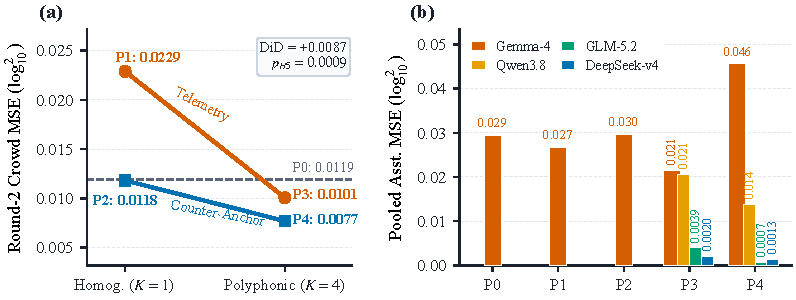
\includegraphics[width=0.92\textwidth]{figures/fig4_factorial_capability.pdf}
  \caption{\textbf{Mixed-model and prompt interventions interact sub-additively, while in-panel model MSE varies $20\times$--$70\times$ across endpoints.} \textbf{(a)}~$2\times 2$ factorial profile ($K\in\{1,4\} \times \text{Framing}$) relative to \texttt{P0} unsocial reference. \textbf{(b)}~Within-panel pooled Round-1+Round-2 assistant MSE ($n=256$ in \texttt{P0}--\texttt{P2}; $n=64$/model in \texttt{P3}--\texttt{P4}) documenting the capability confound.}
  \label{fig:factorial}
\end{figure}

\begin{table}[t]
\centering
\caption{\textbf{Cross-round error expansion (left) and per-model pooled R1+R2 assistant MSE (right).} Best panel accuracy is bolded.}
\label{tab:mechanisms}
\scriptsize
\setlength{\tabcolsep}{3.0pt}
\begin{tabular}{@{}l S[table-format=1.5] S[table-format=1.5] S[table-format=+1.5] S[table-format=1.5] l S[table-format=1.4] S[table-format=1.4] S[table-format=1.4] S[table-format=1.4] S[table-format=1.4]@{}}
\toprule
\textbf{Cond.} & \textbf{$0.36 E_1$} & \textbf{$0.16 E_{a,2}$} & \textbf{$0.48\mathrm{Cross}$} & \textbf{$E_2$ Total} & \textbf{Model} & \textbf{\texttt{P0}} & \textbf{\texttt{P1}} & \textbf{\texttt{P2}} & \textbf{\texttt{P3}} & \textbf{\texttt{P4}} \\
\cmidrule(r){1-5}\cmidrule(l){6-11}
\texttt{P0} & 0.00703 & 0.00154 & +0.00337 & 0.01194 & \texttt{gemma-4-26b} & 0.0294 & 0.0267 & 0.0296 & 0.0215 & 0.0456 \\
\texttt{P1} & 0.01090 & 0.00277 & +0.00923 & 0.02290 & \texttt{qwen3.8-27b} & {---} & {---} & {---} & 0.0205 & 0.0137 \\
\texttt{P2} & 0.00696 & 0.00216 & +0.00270 & 0.01182 & \texttt{glm-5.2}     & {---} & {---} & {---} & 0.0039 & \bfseries 0.0007 \\
\texttt{P3} & 0.00760 & 0.00037 & +0.00208 & 0.01006 & \texttt{deepseek-v4} & {---} & {---} & {---} & \bfseries 0.0020 & 0.0013 \\
\texttt{P4} & 0.00610 & 0.00092 & +0.00066 & \bfseries 0.00769 & \textit{Panel Mean} & 0.0294 & 0.0267 & 0.0296 & 0.0120 & 0.0153 \\
\bottomrule
\end{tabular}
\end{table}

\begin{figure}[t]
  \centering
  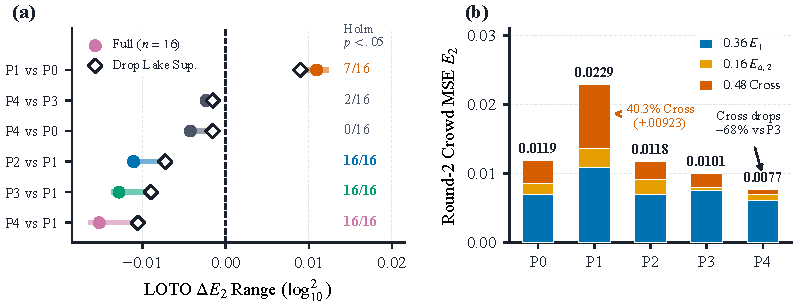
\includegraphics[width=0.92\textwidth]{figures/fig5_loto_crossterm.pdf}
  \caption{\textbf{Rescue contrasts against \texttt{P1} survive all 16 leave-one-task-out drops, and cross-round covariance explains \texttt{P4} vs.\ \texttt{P3}.} \textbf{(a)}~LOTO ($n=15$) diff ranges, full $n=16$ means, and Lake Superior exclusions with $m=9$ Holm survival counts. \textbf{(b)}~Exact Round-2 error shares from~\eqref{eq:cross-term}.}
  \label{fig:loto}
\end{figure}

% ======================================================================
\section{Discussion and Conclusion}
% ======================================================================

Our controlled audit establishes a clear operational distinction for multi-agent epistemics. Inside a homogeneous \texttt{gemma-4-26b-a4b-it} crowd (\texttt{P0}--\texttt{P2}), exposing agents to peer median and IQR telemetry induces strong social herding ($+91.7\%$ MSE, $40.3\%$ cross-round reinforcement), extending persuasion-bias dynamics~\citep{demarzo2003persuasion,kelley2026personalization} to LLM advisory pools. Requiring a concise 53-word bidirectional refutation of both overshoot and undershoot modes (\texttt{P2}) completely eliminates this herding cost ($-48.4\%$, surviving all 16 LOTO drops) while using fewer mean output tokens than naive telemetry ($333.4$ vs.\ $423.8$). Across heterogeneous panels, positive cross-round covariance reduction enables \texttt{P4} to edge below \texttt{P3} on blended crowd MSE ($0.007692$ vs.\ $0.010058$) even when forced counter-anchoring nudges direct Gemma outputs slightly off Frontier consensus; however, sub-additive redundancy ($\mathrm{DiD}=+0.008715$) leaves \texttt{P4 vs P3} statistically unresolved ($p_{\text{H9,ex}}=0.12787$). More broadly, safe multi-agent system design must treat shared consensus interfaces and model-capability mixing as separate hypotheses rather than inferring epistemic diversity benefits without controlled baselines.

% ======================================================================
\section{Limitations and Future Work}
% ======================================================================

Four specific boundaries govern interpretation: (1)~\textbf{Unresolved capability confound:} \texttt{P3} and \texttt{P4} swap $6/8$ Gemma seats for lower-error models; isolating architectural diversity from constituent accuracy and prompt length awaits execution of our implemented follow-up controls (\code{P0\_POLY}, \code{P1\_REFLECT}, and homogeneous DeepSeek/Qwen/GLM arms in~\cref{app:prompts}). (2)~\textbf{Power and single-task leverage:} With $n=16$ tasks ($1$ exact tie), \taskid{hyd\_lake\_superior\_vol\_km3} carries $23\%$--$65\%$ of summed contrast gains, leaving \texttt{P1 vs P0} sensitive to $m=9$ Holm LOTO drops ($7/16$). (3)~\textbf{Synthetic scalar abstraction:} Linear pooling ($\alpha=0.4$), seeded $\pm 0.8$ $\log_{10}$ bias, provider-default sampling, and \texttt{reasoning=\{"effort":"none"\}} abstract away rich natural-language deliberation and human calibration recovery. (4)~\textbf{Runtime token cap override:} \code{providers.py} enforced an $8{,}192$-token minimum vs.\ manifest \code{max\_tokens=1024}, surfacing 14 repetition loops handled via documented retries.\todo{Run pending \code{P0\_POLY}, \code{P1\_REFLECT}, and frontier controls in \code{configs/polyphony\_controls.yaml}.}

% ======================================================================
\section{Dual-Use and Security Considerations}
% ======================================================================

Documenting how compact summary telemetry steers homogeneous agent collectives highlights two dual-use attack surfaces. First, \emph{Sybil or compromised telemetry injection} could plant biased peer medians with narrow IQRs inside forecasting dashboards or multi-agent swarms to shift consensus without triggering safety refusals; practitioners should treat summary telemetry as untrusted input, apply counter-anchoring before pooling, and monitor $D_{\text{excess}}$ and cross-round covariance. Second, indiscriminate anti-consensus forcing risks \emph{weaponized doubt} when calibrated frontier peers already agree (evidenced by Gemma's MSE worsening from $0.0215$ in \texttt{P3} to $0.0456$ in \texttt{P4}); safeguards should therefore trigger only when diversity collapses rather than penalizing justified convergence. All simulated tasks reference public institutional records with zero human subjects, PII, or committed API secrets.

% ======================================================================
\section{Code and Data}
% ======================================================================

All simulation harnesses, the 16-task benchmark (\code{configs/polyphony\_benchmark\_tasks.json}), unrun controls (\code{configs/polyphony\_controls.yaml}), frozen \texttt{P0}--\texttt{P4} responses and HTTP request logs (\code{results/polyphony-p0-p4/}), the superseded 12-task archive (\code{results/polyphony-p0-p4-12task-alpha03/}), and deterministic audit scripts (\code{scripts/audit\_and\_reproduce\_p0\_p4.py}) are publicly archived in the GitHub repository\footnote{\url{https://github.com/vikramwish/apart-epistemics}} (branch \code{numeric-question-bank}, commit \texttt{3a6294c}).

% ======================================================================
\section{Author Contributions}
% ======================================================================

Vikram Viswanath conceived the experimental protocol, selected the 16-task cold-probed benchmark, executed all provider runs, designed and verified all statistical and audit checks, and authored the revised submission.\todo{Update Sec.~9 if co-authors or mentors should be credited.}

% ======================================================================
\section{LLM Usage Statement}
% ======================================================================

AI coding and research assistants assisted with refactoring simulation scripts, implementing deterministic reproduction and permutation audits (\code{scripts/audit\_and\_reproduce\_p0\_p4.py}), generating Matplotlib plotting scripts, formatting \LaTeX{} tables, and verifying primary bibliographic metadata. Every mathematical identity, statistical hypothesis test, claim-to-evidence link, and rendered output was independently executed and verified against \code{results/polyphony-p0-p4/} by the author.

% ======================================================================
% REFERENCES & APPENDICES (Excluded from Main-Text Page Cap)
% ======================================================================
\clearpage
\bibliographystyle{plainnat}
\small
\bibliography{references}
\normalsize

\clearpage
\appendix

\section{Version Resolution, First-Attempt Audit, and Mathematics}\label{app:audit}

An earlier repository commit (\texttt{b5b91ce}, preserved in \code{results/polyphony-p0-p4-12task-alpha03/}) evaluated $12$ tasks at $\alpha=0.3$ ($960$ rows, $979$ calls) and observed flat Round-2 crowd MSE across \texttt{P0}--\texttt{P4} ($0.009932$, $0.010231$, $0.010143$, $0.010340$, and $0.009928$). The target submission reflects the expanded $16$-task, $\alpha=0.4$ experiment (commits \texttt{fdd30fe}/\texttt{3a6294c}, \code{results/polyphony-p0-p4/}). Under~\eqref{eq:cross-term}, unrolled empirical covariance-inclusive variance shares of $0.36\,x_0$ reach $81.90\%$ (\texttt{P0}), $89.17\%$ (\texttt{P1}), $82.83\%$ (\texttt{P2}), $81.89\%$ (\texttt{P3}), and $83.27\%$ (\texttt{P4}); in \texttt{P4}, a $-0.014126$ negative cross term on \taskid{inf\_gbt\_height\_m} lowers positive carry below \texttt{P3}.

\section{16-Task Benchmark, Outcomes, and Extended Sensitivity}\label{app:benchmark}

\Cref{tab:benchmark-full} details all 16 sampled questions, reference truths, institutional sources, misconception polarities ($b_q$), and final Round-2 crowd errors $E_2$ across \texttt{P0}--\texttt{P4}. \Cref{tab:robustness-ext} documents sensitivity to first-pass Wave-1 reconstruction (\taskid{First\_Pass\_Saved\_Pre2328}), strict unretried chronological reconstruction (\taskid{First\_Call\_Ever\_Strict}), institutional source updates (\texttt{S1}--\texttt{S4}), and $n=15$ leave-one-task-out ranges.

\begin{table}[t]
\centering
\caption{\textbf{Complete 16-task benchmark (\code{configs/polyphony\_benchmark\_tasks.json}) and Round-2 crowd MSE $E_2$.} Strata: HS = \code{high\_spread}, LS = \code{low\_spread}, C = \code{control}; $b_q$: misconception polarity (weighted $0.22$). Original benchmark values remain preserved unchanged.}
\label{tab:benchmark-full}
\scriptsize
\setlength{\tabcolsep}{1.8pt}
\begin{tabular}{@{}l c r l S[table-format=-1.1] S[table-format=1.4] S[table-format=1.4] S[table-format=1.4] S[table-format=1.4] S[table-format=1.4]@{}}
\toprule
\textbf{Task ID} & \textbf{Str.} & \textbf{Truth} & \textbf{Primary Institutional Source} & \textbf{$b_q$} & \textbf{\texttt{P0}} & \textbf{\texttt{P1}} & \textbf{\texttt{P2}} & \textbf{\texttt{P3}} & \textbf{\texttt{P4}} \\
\midrule
\taskid{nrg\_us\_hydro\_2023\_twh} & HS & $240\text{ TWh}$ & US EIA Prelim.\ ($245$ final) & -0.8 & 0.0188 & 0.0087 & 0.0042 & 0.0039 & 0.0023 \\
\taskid{sci\_lhc\_dipole\_magnets\_count} & HS & $1{,}232\text{ mag}$ & CERN LHC Specification & -0.8 & 0.0168 & 0.0168 & 0.0168 & 0.0168 & 0.0168 \\
\taskid{hyd\_paijanne\_tunnel\_km} & HS & $120\text{ km}$ & HSY Helsinki Specification & +0.8 & 0.0069 & 0.0125 & 0.0084 & 0.0139 & 0.0107 \\
\taskid{inf\_gbt\_height\_m} & HS & $148\text{ m}$ & NRAO Green Bank ($485\text{ ft}$) & +0.8 & 0.0052 & 0.0427 & 0.0278 & 0.0071 & 0.0016 \\
\taskid{hyd\_delaware\_aqueduct\_km} & HS & $137\text{ km}$ & NYC DEP ($85\text{ mi}$) & +0.8 & 0.0203 & 0.0470 & 0.0245 & 0.0136 & 0.0085 \\
\taskid{nrg\_france\_nuclear\_2022\_twh} & HS & $279\text{ TWh}$ & RTE France Annual Report & -0.8 & 0.0000 & 0.0018 & 0.0010 & 0.0028 & 0.0060 \\
\midrule
\taskid{inf\_elt\_collecting\_area\_m2} & LS & $978\text{ m}^2$ & ESO ELT Optics Spec.\ & +0.8 & 0.0033 & 0.0028 & 0.0016 & 0.0012 & 0.0009 \\
\taskid{mat\_molybdenum\_melting\_c} & LS & $2{,}623\,^\circ\text{C}$ & NIST / CRC ($2{,}896\text{ K}$) & -0.8 & 0.0128 & 0.0148 & 0.0131 & 0.0133 & 0.0125 \\
\taskid{nrg\_us\_wind\_2023\_twh} & LS & $425\text{ TWh}$ & US EIA Electric Power & +0.8 & 0.0104 & 0.0541 & 0.0214 & 0.0228 & 0.0120 \\
\taskid{nrg\_norway\_hydro\_2023\_twh} & LS & $136\text{ TWh}$ & US EIA ($136.1$; SSB $137.3$) & +0.8 & 0.0040 & 0.0162 & 0.0053 & 0.0069 & 0.0055 \\
\taskid{hyd\_murray\_darling\_area\_km2} & LS & $1{,}061{,}469\text{ km}^2$ & MDBA / BoM Statutory & -0.8 & 0.0057 & 0.0060 & 0.0061 & 0.0045 & 0.0041 \\
\taskid{env\_ipcc\_1750\_ch4\_ppb} & LS & $729\text{ ppb}$ & IPCC AR6 WG1 Table~7.4 & -0.8 & 0.0023 & 0.0026 & 0.0022 & 0.0026 & 0.0023 \\
\midrule
\taskid{nrg\_us\_nuclear\_2023\_twh} & C & $775\text{ TWh}$ & US EIA Electric Power & +0.8 & 0.0043 & 0.0079 & 0.0033 & 0.0043 & 0.0035 \\
\taskid{hyd\_lake\_superior\_vol\_km3} & C & $12{,}100\text{ km}^3$ & US EPA / NOAA GLERL & -0.8 & \bfseries 0.0621 & \bfseries 0.1024 & \bfseries 0.0343 & \bfseries 0.0321 & \bfseries 0.0176 \\
\taskid{inf\_snolab\_depth\_m} & C & $2{,}070\text{ m}$ & SNOLAB ($6{,}800\text{ ft}$) & -0.8 & 0.0093 & 0.0149 & 0.0097 & 0.0087 & 0.0134 \\
\taskid{inf\_north\_sea\_link\_km} & C & $720\text{ km}$ & National Grid / Statnett & +0.8 & 0.0089 & 0.0152 & 0.0095 & 0.0065 & 0.0055 \\
\bottomrule
\end{tabular}
\end{table}

\begin{table}[t]
\centering
\caption{\textbf{Extended robustness checks across first-attempt reconstruction, institutional source revisions (\texttt{S1}--\texttt{S4}), and LOTO ($n=15$).} Parentheses report exact $m=9$ Holm-adjusted $p$-values ($p_{\text{H9,ex}}$).}
\label{tab:robustness-ext}
\scriptsize
\setlength{\tabcolsep}{2.4pt}
\begin{tabular}{@{}l c c c c c@{}}
\toprule
\textbf{Sensitivity Variant} & \textbf{\texttt{P1 vs P0}} & \textbf{\texttt{P2 vs P1}} & \textbf{\texttt{P3 vs P1}} & \textbf{\texttt{P4 vs P1}} & \textbf{\texttt{P4 vs P3}} \\
\midrule
Main Retained ($n=16$) & $+0.01096$ ({\tiny .0322}) & $-0.01108$ ({\tiny .0011}) & $-0.01284$ ({\tiny .0093}) & $-0.01521$ ({\tiny .0093}) & $-0.00237$ ({\tiny .1279}) \\
\texttt{First\_Pass\_Saved} & $+0.01307$ ({\tiny .0256}) & $-0.01237$ ({\tiny .0235}) & $-0.01499$ ({\tiny .0077}) & $-0.01736$ ({\tiny .0077}) & $-0.00237$ ({\tiny .1279}) \\
\texttt{First\_Call\_Strict} & $+0.00878$ ({\tiny .1809}) & $-0.01235$ ({\tiny .0299}) & $-0.01488$ ({\tiny .0077}) & $-0.01723$ ({\tiny .0122}) & $-0.00235$ ({\tiny .3330}) \\
\texttt{S1} (EIA US Hydro $245$) & $+0.01091$ ({\tiny .0322}) & $-0.01111$ ({\tiny .0011}) & $-0.01288$ ({\tiny .0093}) & $-0.01526$ ({\tiny .0093}) & $-0.00238$ ({\tiny .1279}) \\
\texttt{S2} (SSB Norway $137.3$) & $+0.01092$ ({\tiny .0322}) & $-0.01105$ ({\tiny .0011}) & $-0.01282$ ({\tiny .0093}) & $-0.01518$ ({\tiny .0093}) & $-0.00236$ ({\tiny .1279}) \\
\texttt{S3} (\texttt{S1} + \texttt{S2}) & $+0.01087$ ({\tiny .0322}) & $-0.01109$ ({\tiny .0011}) & $-0.01285$ ({\tiny .0093}) & $-0.01523$ ({\tiny .0093}) & $-0.00238$ ({\tiny .1279}) \\
\texttt{S4} (Drop Molybd.\ $n=15$) & $+0.01155$ ({\tiny .0513}) & $-0.01171$ ({\tiny .0022}) & $-0.01360$ ({\tiny .0137}) & $-0.01607$ ({\tiny .0137}) & $-0.00247$ ({\tiny .1764}) \\
\texttt{LOTO} $p_{\text{H9}}$ [min--max] & $.0049$--$.0645$ & $.0011$--$.0022$ & $.0049$--$.0186$ & $.0011$--$.0186$ & $.0315$--$.2472$ \\
\texttt{LOTO} $p_{\text{H9}}<0.05$ count & \textbf{7 / 16} ($16/16$ raw) & \textbf{16 / 16} & \textbf{16 / 16} & \textbf{16 / 16} & \textbf{2 / 16} ($16/16$ raw) \\
\bottomrule
\end{tabular}
\end{table}

\section{Prompt Templates and Follow-Up Controls}\label{app:prompts}

\Cref{tab:control-roadmap} summarizes the implemented follow-up controls in \code{configs/polyphony\_controls.yaml}. Below are the exact runtime prompt templates defined in \code{src/apart\_epistemics/engine/numeric\_core.py}:
\begin{itemize}
  \item \textbf{System instruction (all conditions):} \emph{``You are a quantitative scientific estimator. Answer without web lookup and end with `Final estimate: <number>'. Today's date is 2026-11-15.''}
  \item \textbf{Social telemetry snippet (\texttt{P1}--\texttt{P4}):} \emph{``Peer consensus telemetry from prior estimators reports a median of \{med\} (interquartile range \{q25\} to \{q75\}).''}
  \item \textbf{Dialectical counter-anchoring block (\texttt{P2}, \texttt{P4}; 53 words):} \emph{``Dialectical counter-anchoring protocol: before estimating, write 2-3 concise sentences testing both tails --- identify specific physical scaling mechanisms or misconceptions by which both the prior estimate and peer median could systematically overshoot (too high) OR undershoot (too low) the true value --- then derive your estimate from independent physical principles and reference scales.''}
  \item \textbf{Matched neutral verification block (\texttt{P1\_REFLECT} control; 51 words):} \emph{``Structured verification protocol: before estimating, write 2-3 concise sentences checking the quantity carefully --- verify exact unit definitions, confirm any geographical or historical time bounds, and audit each step of intermediate arithmetic to ensure clear order-of-magnitude plausibility --- then derive your final estimate directly from verified physical principles and reference scales.''}
\end{itemize}

\begin{table}[t]
\centering
\caption{\textbf{Implemented (unrun) follow-up control matrix in \code{configs/polyphony\_controls.yaml} ($8$ agents $\times 2$ rounds $\times 16$ tasks).}}
\label{tab:control-roadmap}
\scriptsize
\setlength{\tabcolsep}{3.0pt}
\begin{tabular}{@{}l c l l l@{}}
\toprule
\textbf{Control Arm} & \textbf{$K$} & \textbf{Composition} & \textbf{Telemetry / Prompt} & \textbf{Confound Isolated} \\
\midrule
\code{P0\_POLY} & 4 & $2\times$\{\texttt{gemma-4}, \texttt{ds-v4}, \texttt{qwen3.8}, \texttt{glm-5.2}\} & Unsocial / Neutral & Silent 4-model ensemble vs.\ \texttt{P3}/\texttt{P4} \\
\code{P1\_REFLECT} & 1 & $8\times$\texttt{gemma-4-26b-a4b-it} & Median+IQR / 51-wd Verify & Counter-anchoring vs.\ reflection length \\
\code{P0\_DS}, \code{P1\_DS} & 1 & $8\times$\texttt{deepseek-v4-flash} & Unsocial / Social Neutral & DeepSeek capability \& herding \\
\code{P0\_QWEN}, \code{P1\_QWEN} & 1 & $8\times$\texttt{qwen3.8-27b} & Unsocial / Social Neutral & Qwen capability \& herding \\
\code{P0\_GLM}, \code{P1\_GLM} & 1 & $8\times$\texttt{glm-5.2} & Unsocial / Social Neutral & GLM capability \& herding \\
\bottomrule
\end{tabular}
\end{table}

\end{document}
